\documentclass{article}
\usepackage[inline]{enumitem}
\usepackage{lipsum}
\usepackage[magyar]{babel}
\usepackage{graphicx}
\usepackage{subcaption}


\begin{document}
\listoffigures
\newpage

\begin{enumerate}
\item egy
\item kettő
\item[és] három
\end{enumerate}

\begin{enumerate}
\item Első szint
\item Első szint
\item Első szint
\begin{itemize}
\item Második szint
\item Második szint
\item Második szint
\begin{itemize}
\item Harmadik szint
\item Harmadik szint
\item Harmadik szint
\begin{itemize}
\item Negyedik szint
\item Negyedik szint
\item Negyedik szint 
\begin{itemize}
\item Ötödik szint
\item Ötödik szint
\item Ötödik szint 
\begin{enumerate}[label=$\int$]
\item Hatodik szint
\item Hatodik szint
\item Hatodik szint 
\end{enumerate}

\end{itemize}
\end{itemize}
\end{itemize}
\end{itemize}
\end{enumerate}

\lipsum[1-2]
\begin{enumerate}[resume,label=$\int$]
\item[] Hatodik szint \label{} \ref{}
\item Hatodik szint \label{} \ref{}
\end{enumerate}

\begin{description}[align=parleft,leftmargin=*,widest={hosszabb}]
\item[címke] \lipsum[1]
\item \lipsum[2]
\item[ez egy hosszabb címke] \lipsum[3]
\end{description}


\begin{figure}[bt]
\centering
\caption{Felirat/Képaláírás}
\hspace{1em} % vízszintes helykihagyás

\begin{subfigure}{5cm}
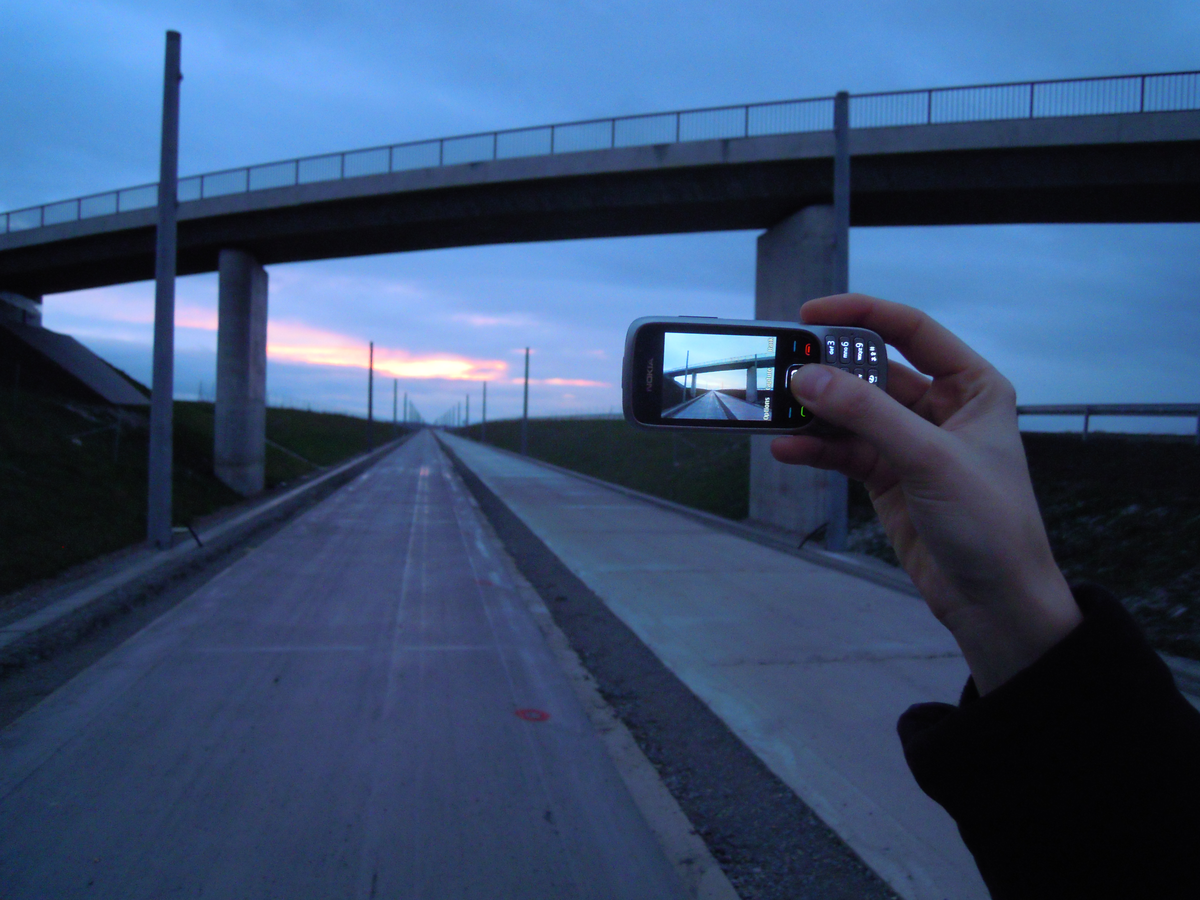
\includegraphics[width=.4\linewidth]{image.png}
\label{felirat}
\caption{szöveg}
\end{subfigure}

\begin{subfigure}{5cm}
\scalebox{1}[-1]{
\includegraphics[width=.7\linewidth]{image2.jpg}}
\caption{tülrözött kép}
\label{fig:kepek}
\end{subfigure}
\lipsum

\end{figure}

\newpage
\begin{tabular}{r|ll}

\end{tabular}


\end{document}

